
\chapter{Steganografia}\label{chap:steganography}
{
    % - czym jest steganografia
    % - odniesienie do kryptografii
    % - rys historyczny
    %   - pierwsze użycia w starożytności
    %   - przykłady
    % - steganografia cyfrowa (jakiś diagram idk), opis mediów nośnych
    % - steganografia z wykorzystaniem obrazów
    %   - podział na techniki dziedzinowe i przestrzenne
    %   - opis metod (LSB etc)
    %   - vLSB
    %   - wpływ doboru obszaru na pojemność obrazu

    % CO TO STEGANOGRAFIA
    Steganografia jest dziedziną nauki poświęconą ukrywaniu informacji w jawnych kanałach komunikacji. Nazwa nauki
    wywodzi się z języka greckiego, i może być tłumaczona jako ,,ukryte pismo'' (\textit{steganós} - ukryty,
    \textit{graphia} - pismo).

    % CO TO KRYPTOGRAFIA
    W celu podkreślenia cech oraz charakteru metod steganograficznych często przytaczane jest również pojęcie
    kryptografii. Obiektem zainteresowań kryptografii jest uniemożliwienie zrozumienia treści wiadomości przez osoby
    postronne, pozbawione do niej dostępu. Współcześnie jest to osiągane poprzez stosowanie klucza dzielonego przez
    osoby zaufane (kryptografia symetryczna) lub par kluczy publicznych i prywatnych (kryptografia asymetryczna). Dzięki
    ich zastosowaniu, osoba postronna pomimo dostępu do szyfrogramu nie jest w stanie wydobyć tekstu jawnego.

    % CZYM SIĘ RÓŻNIĄ
    W odróżnieniu od kryptografii, celem technik steganograficznych jest umożliwienie uczestnikom komunikacji
    przesyłania informacji bez ujawniania faktu istnienia samego przekazu.
    
    \section{Zastosowania steganografii}
    {
        % PRZYKŁADY HISTORYCZNE
        Pierwszych przykładów zastosowania steganografii można doszukiwać się już w czasach
        starożytnych\cite{Petitcolas1999InformationHS}. Herodotus, w swoim dziele \textit{Dzieje} opisuje historię
        greckiego polityka Histiajosa, który w celu przekazania poufnej informacji wytatuował ją na skalpie zaufanego
        niewolnika. Gdy jego włosy odrosły, został on wysłany w celu doręczenia listu oraz ukrytej wiadomości. Do innych
        przykładów steganografii można zaliczyć również ukrywanie wiadomości w zapisach nutowych, stosowanie atramentów
        sympatycznych lub technikę mikrokropek\cite{Petitcolas1999InformationHS}, która przeżyła swój renesans w czasach
        zimnej i drugiej wojny światowej.

        % WSPÓŁCZESNE ZASTOSOWANIA STEGANOGRAFII
        Warto również podkreślić, że kolejnym z zastosowań steganografii są znaki wodne oraz symbole pozwalające na
        identyfikację źródła informacji. Za równo w przypadku multimediów objętych prawami autorskimi jak i poufnych
        dokumentów, ich producent lub organizacja strzegąca ich tajności może umieścić ukryte informacje pozwalające
        wskazać źródło wycieku\cite{Nasereddin2011DIGITALWA}. Podobną technikę stosują producenci drukarek - seria oraz
        model drukarki może być odzwierciedlona w drukowanym dokumencie poprzez układ niewidocznych gołym okiem żółtych
        kropek. Takie działania mają na celu ułatwienia walki z przestępczością polegającą na fałszowaniu dokumentów i
        banknotów\cite{Richter2018ForensicAA}.
    }

    \section{Steganografia cyfrowa}
    {
        % STEGANOGRAFIA CYFROWA
        Wraz z wzrostem wykorzystania komputerów do celach multimedialnych oraz rozpowszechnieniu szerokopasmowego
        internetu coraz popularniejsza i bardziej opłacalna staje się steganografia cyfrowa. Jej ideą jest wykorzystanie
        jako medium nośnego różnych rodzajów plików komputerowych lub protokołów komunikacji cyfrowej. Przykładem
        wykorzystania protokołów do celów steganograficznych może być ukrywanie danych w polach kontrolnych ramek
        TCP/IP, kontrolowanie opóźnień między poszczególnymi pakietami lub nawet umyślne powodowanie utrat wybranych
        pakietów\cite{DataHidinginTCP}.

        % STEGANOGRAFIA W PLIKACH MULTIMEDIALNYCH
        Znacznie prostszą, lecz bardzo rozwiniętą techniką jest wykorzystanie plików multimedialnych takich jak zdjęcia,
        pliki muzyczne i filmy. Do ich szczególnej atrakcyjności jako medium służące do ukrywania informacji przyczynia
        się między innymi ich wszechobecność, duże rozmiary oraz wysoka nadmiarowość\cite{Mitchell2018H264ED,
        Pope2012DigitalS}. Ostatni aspekt w kontekście steganografii ma szczególne znaczenie, gdyż oznacza że
        modyfikacja pewnej części informacji bitowej zawartej w pliku ma niski wpływ na jego końcową treść. Przykładowo,
        zmiana wartości jednego z kanałów konkretnego piksela będzie miało mało zauważalny wpływ na końcowy obraz nawet
        przez uważnego obserwatora. Podobne prawidłowości można również dostrzec w plikach muzycznych - manipulacja
        zawartością częstotliwości składowych będących poza granicą percepcji, czyli poniżej 20Hz i powyżej 20kHz
        również będzie trudna w detekcji przez subiektywnego odbiorcę\cite{Wheeler2012AudioSU}. Innym przykładem
        ukrywania informacji w muzyce jest tzw. \textit{backmasking}, polegający na ukrywaniu wiadomości możliwych w
        odbiorze tylko i wyłącznie po odtworzeniu utworu od tyłu. Jednym z pierwszych zespołów przyczyniających się do
        wzrostu popularności powyższych eksperymentów jest \textit{The Beatles}.
    }
    
    \section{Steganografia z wykorzystaniem obrazów cyfrowych}
    {
        % TECHNIKI UKRYWANIA INFORMACJI W OBRAZACH
        Mimo tego, że jako medium steganograficzne można wykorzystać każdy plik binarny, szczególnie dużo uwagi zostało
        poświęcone cyfrowym obrazom i zdjęciom. Pomimo pozornej prostoty powyższego zadania powstało wiele
        wyrafinowanych metod i technik, różniących się za równo pod kątem założeń jak i rezultatów. Pierwszym parametrem
        mogącym służyć do podziału zaproponowanych metod jest dziedzina w której  obraz zostaje poddany analizie. 

        \subsection{Techniki przestrzenne}
        {
            % TECHNIKI PRZESTRZENNE
            W technikach przestrzennych, obraz jest traktowany jak zbiór punktów (pikseli) umieszczonych w dwuwymiarowym
            układzie współrzędnych. Zaletą tych metod jest ich intuicyjność oraz przystępność, lecz są to również metody
            bardziej podatne na ataki polegające na wykryciu lub zniszczeniu ukrytej wiadomości\cite{Sharma2020AnIS}.

            % LSB
            Najbardziej powszechną techniką przestrzenną jest metoda \textit{Least Significant Bit (LSB)}. Jej
            zastosowanie  sprowadza się do zastąpienia najmniej znaczącego bitu obrazu będącego nośnikiem informacji
            bitem wiadomości  ukrywanej. W zależności od spadku jakości który uznajemy za akceptowalny, możemy
            wykorzystać \textit{n} najmniej  znaczących bitów każdego z kanałów \textit{RGB}. Pewnym uszczegółowieniem
            \textit{LSB} jest metoda  \textit{4LSB}. Zakłada ona wykorzystanie dokładnie 4 bitów z każdego bajtu obrazu
            maskującego, co przekłada się  na wykorzystanie 50\% pojemności nośnika. Kosztem tak znacznej pojemności
            jest znaczący spadek jakości obrazu  oraz ułatwiona steganoanaliza.

            % VLS
            W celu zmniejszenia wykrywalności manipulacji obrazu przy jednoczesnym zachowaniu względnie dużej pojemności
            steganogramu, zaproponowano technikę \textit{Variable Least Significant Bit
            (VLSB)}\cite{Khan2011ImplementationOV}. W przeciwieństwie do \textit{LSB} podczas ukrywania danych
            wykorzystywana jest różna ilość bitów obrazu w zależności od położenia piksela. Nośnik zostaje podzielony na
            zadaną ilość sekcji, a następnie dla każdej z nich wyznaczana jest ilość bitów które zostaną zastąpione
            tekstem  jawnym. Twórcy metody zaproponowali algorytm \textit{Decreasing Distance Decreasing Bits Algorithm
            (DDDBA)},  który na podstawie odległości sektora względem piksela referencyjnego, którym najczęściej jest
            środkowy piksel  obrazu, wyznacza proporcjonalną ilość ukrywanych bitów. Wynikiem działania algorytmu
            \textit{VLSB} jest obraz,  którego środkowa część jest mniej zniekształcona, co obniża subiektywne odczucie
            spadku jakości i pozwala na  ukrycie większej ilości danych\cite{Khan2011ImplementationOV}.

            % VIVBS
            Dalszym udoskonaleniem, za równo pod kątem bezpieczeństwa ukrywanej informacji jak i utrudnienia
            wykrywalności  ukrytego przekazu jest metoda o nazwie \textit{Varying Index Varying Bits Substitution
            (VIVBS)} zaproponowana  przez Sahib Khan, N. Ahmad i M. Wahid\cite{Khan2016VaryingIV}. Podobnie jak w
            metodzie \textit{VLSB}, ilość  wykorzystanych bitów obrazu nośnego jest zmienna. W przeciwieństwie do
            wariantu \textit{VLSB} opartego o  algorytm \textit{DDDBA}, ilość bitów ukrywanych w danym pikselu nie jest
            wyznaczana podczas działania algorytmu,  lecz jest zależna od dodatkowego klucza będącego parametrem jego
            działania. Klucz przyjmuje postać tablicy  przypisującej indeksowi każdego z pikseli ilość bitów które
            należy zastąpić bitami tekstu jawnego. Ponieważ  ilość możliwych kombinacji rozmieszczenia bitów informacji
            w obrazie jest znacząca, odczytanie przekazu poprzez  wykorzystanie przeszukiwania wyczerpującego poprzez
            osobę postronną nieposiadającą klucza będzie praktycznie  niemożliwe. Główną wadą, powyższej metody jest jej
            również największa zaleta - klucz definiujący rozmieszczenie  informacji w pikselach obrazu. Każdorazowe
            kodowanie informacji wymaga utworzenia klucza, od którego będzie  również zależeć wpływ procesu na jakość
            obrazu - arbitralny wybór wysokiej ilości wykorzystanych bitów w  nieodpowiednich sekcjach obrazu może
            przykuć uwagę osób postronnych i zdradzić fakt istnienia ukrytego przekazu.  Dodatkową wadę metody jest
            również rozmiar klucza -  w minimalnym przypadku, w którym wykorzystujemy 0 lub 1 bit  każdego piksela klucz
            ma rozmiar $w * h$ bitów, gdzie \textit{w} i \textit{h} to odpowiednio szerokość i  wysokość obrazu. Wraz z
            wzrostem ilości wykorzystywanych bitów, rozmiar klucza również będzie się
            powiększał\cite{Khan2016VaryingIV}.

            % VPD
            W celu poprawy subiektywnej oceny jakości obrazów oraz zmniejszenia ryzyka przekazu w roku 2003, Da-Chun Wu
            oraz  W. Tsai zaproponowali metodę \textit{Value Pixel Differencing (VPD)}. Jednym z jej założeń jest
            uzależnienie  ilości wykorzystanych bitów obrazu nośnego od różnicy pomiędzy poziomami intensywności
            kolejnych  pikseli\cite{Wu2003ASM}. W metodzie \textit{VPD} piksele są odczytywane parami sekwencyjnie,
            zakreślając ciągły,  łamany kształt. Dla każdej napotkanej pary pikseli obliczana jest ich różnica jasności,
            a następnie na jej  podstawie wyznaczana jest ilość bitów które zostaną podmienione na treść ukrywanej
            wartości. Ilość ukrytych  bitów jest proporcjonalna do zmiany wartości pikseli. W ten sposób możliwe jest
            osiągnięcie obrazów mniej  podatnych na steganoanalizę przy jednoczesnym zachowaniu znacznej
            pojemności\cite{Wu2003ASM}.
            
        }

        \subsection{Techniki częstotliwościowe}
        {
            % CO TO
            Alternatywnym podejściem do steganografii wykorzystującej cyfrowe obrazy, są techniki oparte o
            częstotliwościową reprezentację obrazów. Metody te polegają na transformacji obrazu w postaci bitmapy do
            macierzy współczynników określających amplitudę lub natężenie fal o konkretnych częstotliwościach
            występujących w obrazie\cite{ImageCompressionDCT, Reichel2001IntegerWT}.

            % PO CO
            Analiza obrazów w dziedzinie częstotliwości daje alternatywną perspektywę na treść obrazu i pozawala na
            rozpoznawanie, ekstrakcję i manipulację poszczególnych cech które mają odmienny wpływ na jego percepcję.
            Pasma niskich częstotliwości przekładają się na percepcję ogólnych kształtów i barw obiektów oraz ich
            kompozycję i wzajemne umiejscowienie. Pasma wysokie pozwalają na rozróżnianie ostrych krawędzi obrazów,
            rozpoznawanie detali oraz reprezentują wszelkie złożone tekstury\cite{ImageSpatialFreq}.

            % WATERMARKING
            Metody częstotliwościowe zyskały również na popularności w pokrewnej dziedzinie do steganografii, jaką jest
            oznaczanie (ang. \textit{watermarking}) produktów cyfrowych. Za równo ukrywając dane poufne, jak i cyfrowe
            podpisy chroniące praw autorskich, celem metod działających w dziedzinie częstotliwościowej jest nie tylko
            zachowanie możliwie najwyższej jakości medium w którym zawarto dodatkowe informacje, lecz również
            uodpornienie ukrytego przekazu na jego manipulację i zniszczenie przez kompresję\cite{Tao2014RobustIW}.

            % DCT
            Jedną z transformat pozwalających na wyznaczenie częstotliwościowej reprezentacji obrazu jest
            \textit{Dyskretna transformata kosinusowa (DCT)}\cite{ImageCompressionDCT}. Polega ona na podziale obrazu na
            bloki, najczęściej rozmiaru 8x8 pikseli. Następnie wyznaczana jest macierz współczynników $T_{i, j}$ za
            pomocą poniższego wzoru \ref{eqt:dctcoef}. $N$ oznacza rozmiar bloku, w powszechnych zastosowaniach wynosi
            8.

            \begin{equation}\label{eqt:dctcoef}
                T_{i, j}=\left\{\begin{array}{ll}\frac{1}{\sqrt{N}} & \text { if } i=0 \\ \sqrt{\frac{2}{N}} \cos \left[\frac{(2 j+1) i \pi}{2 N}\right] & \text { if } i>0\end{array}\right\}
            \end{equation}
            
            W kontekście złożoności obliczeniowej istotny jest fakt, że macierz transformacji $T$ można wyznaczyć
            jednokrotnie i ponownie wykorzystać dla każdego z bloków obrazu. W tym przypadku stosowane jest równanie
            \ref{eqt:dctmat}, w którym wyznacza się macierz współczynników $D$ korzystając z macierzy transformacji $T$
            oraz bloku wartości pikseli $M$ przeskalowanych do zakresu $[-128, 127]$.
            
            \begin{equation}\label{eqt:dctmat}
                D=T M T^{\prime}
            \end{equation}
            
            Jednym z zastosowań dyskretnej transformacji kosinusowej jest stratna kompresja danych, przykładowo w
            formacie JPEG. Po wyznaczeniu współczynników odpowiadających kolejnym częstotliwościom następuje proces
            kwantyzacji - macierz współczynników zostaje skalarnie przemnożona przez macierz kwantyzacji a następnie
            zaokrąglana. Zadaniem macierzy kwantyzacji jest przeskalowanie współczynników odpowiadających zakresom
            częstotliwości w taki sposób, aby pasma których zmiany mają najmniejszy wpływ na subiektywną percepcję
            przyjęły wartości bliskie zeru. Ostatnim krokiem kompresji jest zaokrąglenie uzyskanych współczynników.
            Poprzez odrzucenie miejsc po przecinku wszystkich współczynników końcowy obraz charakteryzuje się dużo
            mniejszym rozmiarem. W celu rekonstrukcji wykonuje się transformację odwrotną (\textit{IDCT}).

            % DCT - PRZYKŁADY
            Przykładem algorytmu steganograficznego korzystającego z \textit{DCT} jest praca ,,Reversible Data Hiding in
            JPEG Images''\cite{Huang2016ReversibleDH, Li2007ASM}. Wyznaczone współczynniki częstotliwości służą za
            nośnik tekstu jawnego - współczynnikom z eksperymentalnie dobranych pasm częstotliwości zostają podmienione
            najmniej znaczące bity, podobnie jak w przestrzennych metodach \textit{LSB}. W celu osiągnięcia dużo
            większej odporności steganogramu na kompresję, Zhiqiang Zhu, N. Zheng, Tong Qiao oraz Ming Xu zaproponowali
            metodę opartą o manipulację znaków współczynników, w odróżnieniu do manipulacji ich
            wartościami\cite{Zhu2019RobustSB}.

            % DWT + IWT
            Inną transformacją wykorzystywaną w steganografii jest \textit{Dyskretna transformata falkowa} (ang.
            \textit{Discrete wavelet transform (DWT)}) oraz jej odpowiednik pozwalający na bezstratną transformację
            odwrotną - \textit{Całkowitoliczbowa transformata falkowa} (ang. \textit{Integer wavelet transform
            (IWT)})\cite{Xuan2005LosslessDH}.
            
            Jedną z możliwości transformaty falkowej jest wyodrębnienie części obrazu w której skład wchodzą osobno
            wysokie i niskie pasma częstotliwości. Obraz zostaje kolejno przekształcany wierszami i kolumnami przez
            filtr dolnoprzepustowy (wykonujący operację uśredniania) i górnoprzepustowy (obliczający różnicę).
            
            Po pierwszej iteracji oryginalny obraz zostaje podzielony na sekcje:
            \begin{itemize}
                \item LL - filter dolnoprzepustowy zaaplikowany do wierszy i kolumn,
                \item LH - filter dolnoprzepustowy zaaplikowany do wierszy, górnoprzepustowy dla kolumn,
                \item HL - filter górnoprzepustowy zaaplikowany do wierszy, dolnoprzepustowy dla kolumn,
                \item HH - filter górnoprzepustowy zaaplikowany do wierszy i kolumn.
            \end{itemize}

            Przykład działania \textit{IWT} przedstawia rysunek \ref{fig:iwtdemo}.

            \begin{figure}
                \centering
                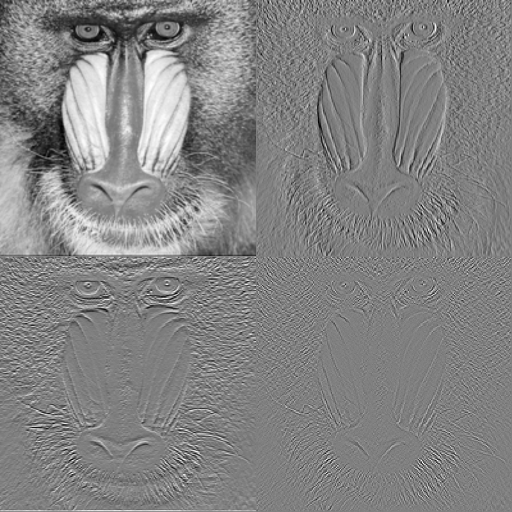
\includegraphics[scale=0.5]{IntegerWaveletTransformDemo}
                \caption{Wynik działania \textit{IWT} na przykładowym obrazie. Kolejno sekcje LL, HL, LH, HH. Do wykonania
                    rysunku wykorzystano narzędzie Image Processing Online Demonstration,
                    http://bigwww.epfl.ch/demo/ip/demos/wavelets/}
                \label{fig:iwtdemo}
            \end{figure}
            

            W artykule ,,Lossless Data Hiding Using Integer Wavelet Transform and Threshold Embedding Technique''
            opisano metodę ukrywania bitów wiadomości w najmniej znaczących bitach współczynników odpowiadających pasmom
            wysokiej częstotliwości. Wyniki eksperymentalne, względem innych metod, wykazały znaczący wzrost pojemności
            obrazu przy zachowaniu tego samego współczynnika szczytowego stosunku sygnału do
            szumu\cite{Xuan2005LosslessDH}.
        }

        \subsection{Podsumowanie}
        {
            % WYKORZYSTANIE ZŁOŻONYCH OBSZARÓW OBRAZÓW
            Na podstawie przytoczonej literatury oraz opisanych metod, można zauważyć pewną tendencję sugerującą
            istotność doboru regionów obrazu w których są ukrywane dane. W opisanych pracach korzystających z
            transformat częstotliwościowych, dokonywano wyboru pomiędzy ukrywaniem danych w
            niskich-średnich\cite{Huang2000EmbeddingIW, DataHidinginJPEG, Li2007ASM} lub wysokich pasmach
            częstotliwości\cite{Xuan2005LosslessDH, Muhuri2020ANI}. 
            
            Główną motywacją autorów decydujących się na dobór niskich bądź średnich pasm w celach ukrywania informacji
            jest uzyskanie obrazu o większej odporności na manipulacje i zniekształcenia. W pracach opisujących metody
            wykorzystujące wysokie pasma częstotliwości, wybór jest argumentowany niższą percepcyjną wykrywalnością
            przez osobę postronną.

            Mechanizm ludzkiej percepcji obrazów jest niezmiernie złożony a nauki z nią związane pozostają dziedzinami w
            których pozostaje jeszcze wiele do odkrycia i wyjaśnienia. Na postrzeganie i rozróżnianie obrazów wpływa nie
            tylko udział poszczególnych składowych częstotliwości, lecz również stosunek kontrastu pasm oraz sposoby
            uprzedniego przetwarzania obrazu\cite{Perfetto2020EffectsOS}. Niemniej jednak, eksperymentalne badania
            przeprowadzane na grupie uczestników sugerują większe znaczenie niższych i średnich pasm częstotliwości przy
            percepcji jakości oraz zniekształceń obrazów. Dowodem tego mogą być powszechnie stosowane tablice
            kwantyzacji wykorzystywane w formatach stratnej kompresji, które faworyzują pasma o średniej lub niższej
            częstotliwości\cite{ImageCompressionDCT}. Oznacza to, że istnieje większy potencjał w manipulacjach obrazem
            w zakresie pasm wysokich, przy jednoczesnej zachowaniu jak najwyższej subiektywnej jakości obrazu. Istnieją
            prace związane z steganografią popierające powyższą tezę. Należą do nich już przytoczona w kontekście metody
            \textit{PVD} ,,A steganographic method for images by pixel-value differencing"\cite{Wu2003ASM}, oraz
            praca,,Edge-based image steganography''  oparta na wykrywaniu krawędzi obrazu\cite{Islam2014EdgebasedIS}.
        }
    }
}

% steganogram - nośnik + ukrywana wiadomość
% steganoanaliza - proces wykrywania i ekstrakcji tekstu jawnego
% stegokanał - kanał przesyłu ukrytej informacji

% TECHNIKI CZĘSTOTLIWOŚCIOWE
% file:///Users/grzegorzkazana/Desktop/Stegano_Ant/IntegerWaveletTransform.pdf
% file:///Users/grzegorzkazana/Desktop/Stegano_Ant/DiscreteCosineTransform.pdf
% file:///Users/grzegorzkazana/Desktop/Stegano_Ant/A%20Novel%20Image%20Steganographic%20Method%20based%20on%20Integer%20Wavelet%20Transformation%20and%20Particle%20Swarm%20Optimization.pdf
% file:///Users/grzegorzkazana/Desktop/Stegano_Ant/A%20steganographic%20method%20based%20upon%20JPEG%20and%20particle%20swarm%20optimization%20algorithm.pdf


% PRACE WSPOMINAJĄCE O UKRYWANIU W 'COMPLEX REGIONS'
% file:///Users/grzegorzkazana/Desktop/Stegano_Ant/ASteganographicMethodForImagesByPixelValueDifferencing.pdf
% file:///Users/grzegorzkazana/Desktop/Stegano_Ant/Ant%20Colony%20Optimization%20ACO%20based%20Data%20Hiding%20in%20Image%20Complex%20Region.pdf
% file:///Users/grzegorzkazana/Desktop/Stegano_Ant/Edge-based_image_steganography.pdf
% file:///Users/grzegorzkazana/Desktop/Stegano_Ant/ICME05-Lossless20Data20Hiding20Using20Integer20Wavelet20Transform20and20Threshold20Embedding20Technique.pdf - Xuan2005LosslessDH

% dobra prezka z AGH o IWT http://home.agh.edu.pl/~jsw/oso/FT.pdf
